\documentclass{standalone}
\usepackage{tikz}
\begin{document}


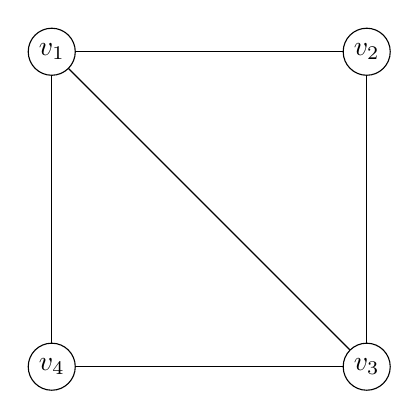
\begin{tikzpicture}[scale=2]
\tikzstyle{vertex}=[circle, draw, minimum size=17pt, inner sep=0pt]
\node[vertex] (V1) at (0,2) {$v_1$};
\node[vertex] (V2) at (2,2) {$v_2$};
\node[vertex] (V3) at (2,0) {$v_3$};
\node[vertex] (V4) at (0,0) {$v_4$};

\path 
(V1) edge (V2)
    edge (V4)
    edge (V3)
(V3) edge (V2)
    edge (V4);y

\end{tikzpicture}

\end{document}
